The octree browsing, no matter if this is the scene octree or a mesh octree,
the dummy implementation is to loop over \textsc{subnodeOffsets}
(Figure~\ref{code:octree_node_struct}), and if there is a children, test if
there is an intersection with the current ray. But on the iterative octree
browsing algorithm, that means more loop iterations, for iterations as useless
as testing if there is a children node. That means more code nested in a if
statement in this loop, and therefore an overall probability even smaller that
threads wants to executes the same instruction, decreasing the warp efficiency.
The idea of this optimization is to compute list of available sub-nodes in
a given node. But since we want to browse the octree in the direction of the
ray to keep the depth test on octree nodes, that means we need 8 of those list,
because of the $2^3 = 8$ differences ray's component's sign combinations.

\begin{figure}[H]
    \centering
    \begin{lstlisting}[morekeywords={uint8_t,uint32_t}]
struct octree_node_t
{
    // the sub-nodes' offset from the octree root
    uint32_t subnodeOffsets[8];
    // the first primitive (mesh or triangle) id
    uint32_t primFirst;
    // the number of primitives
    uint32_t primCount;
    // raw sub-node access lists
    uint32_t subnodeAccessLists[8];
    // the node's sub-node count
    uint8_t subnodeCount;
};
    \end{lstlisting}
    \caption{Octree node's structure with raw access lists.}
    \label{code:raw_access_list}
\end{figure}

And we can actually witness that the number of iterations for each ray is
then greatly reduce as Figures~\ref{fig:stanford_dragon_without_access_list} and
\ref{fig:stanford_dragon_with_access_list} show.

\begin{figure}[h]
    \centering
    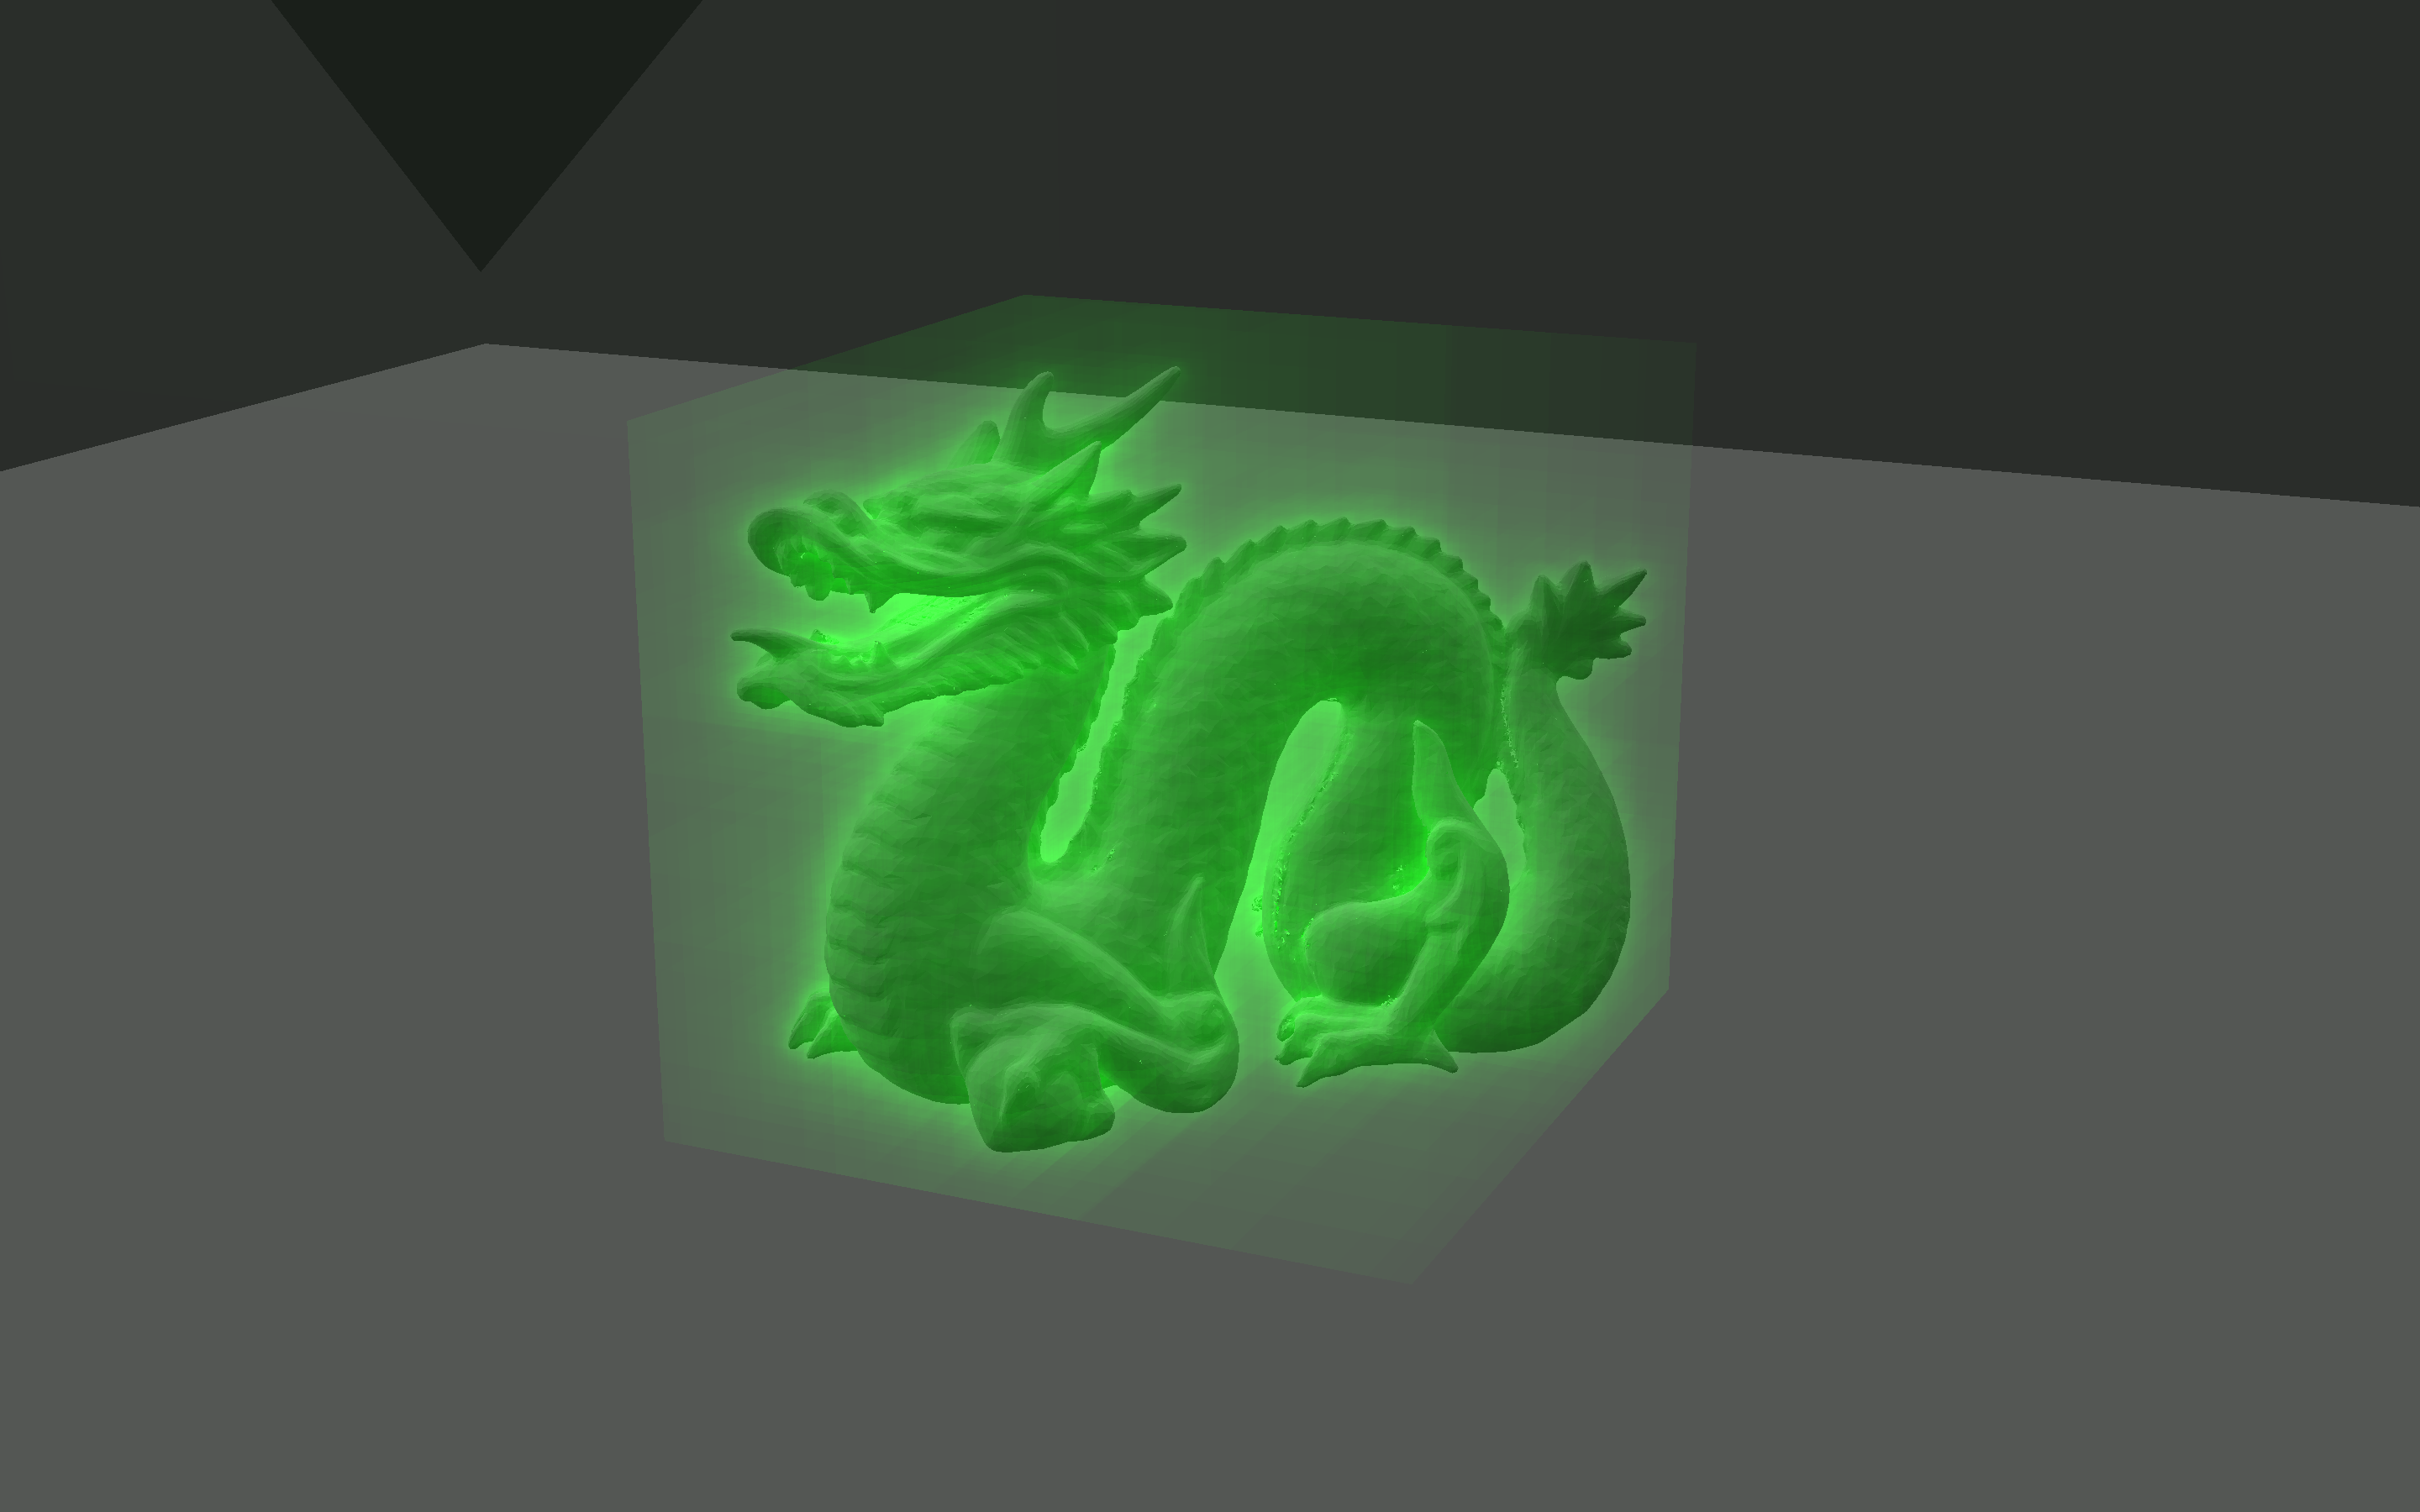
\includegraphics[width=0.8\columnwidth]{stats_octree_loops.png}
    \caption{
        Stanford dragon rendered without the sub-node access lists showing
        the linear number of octree loops required to browse.
    }
    \label{fig:stanford_dragon_without_access_list}
\end{figure}

\begin{figure}[h]
    \centering
    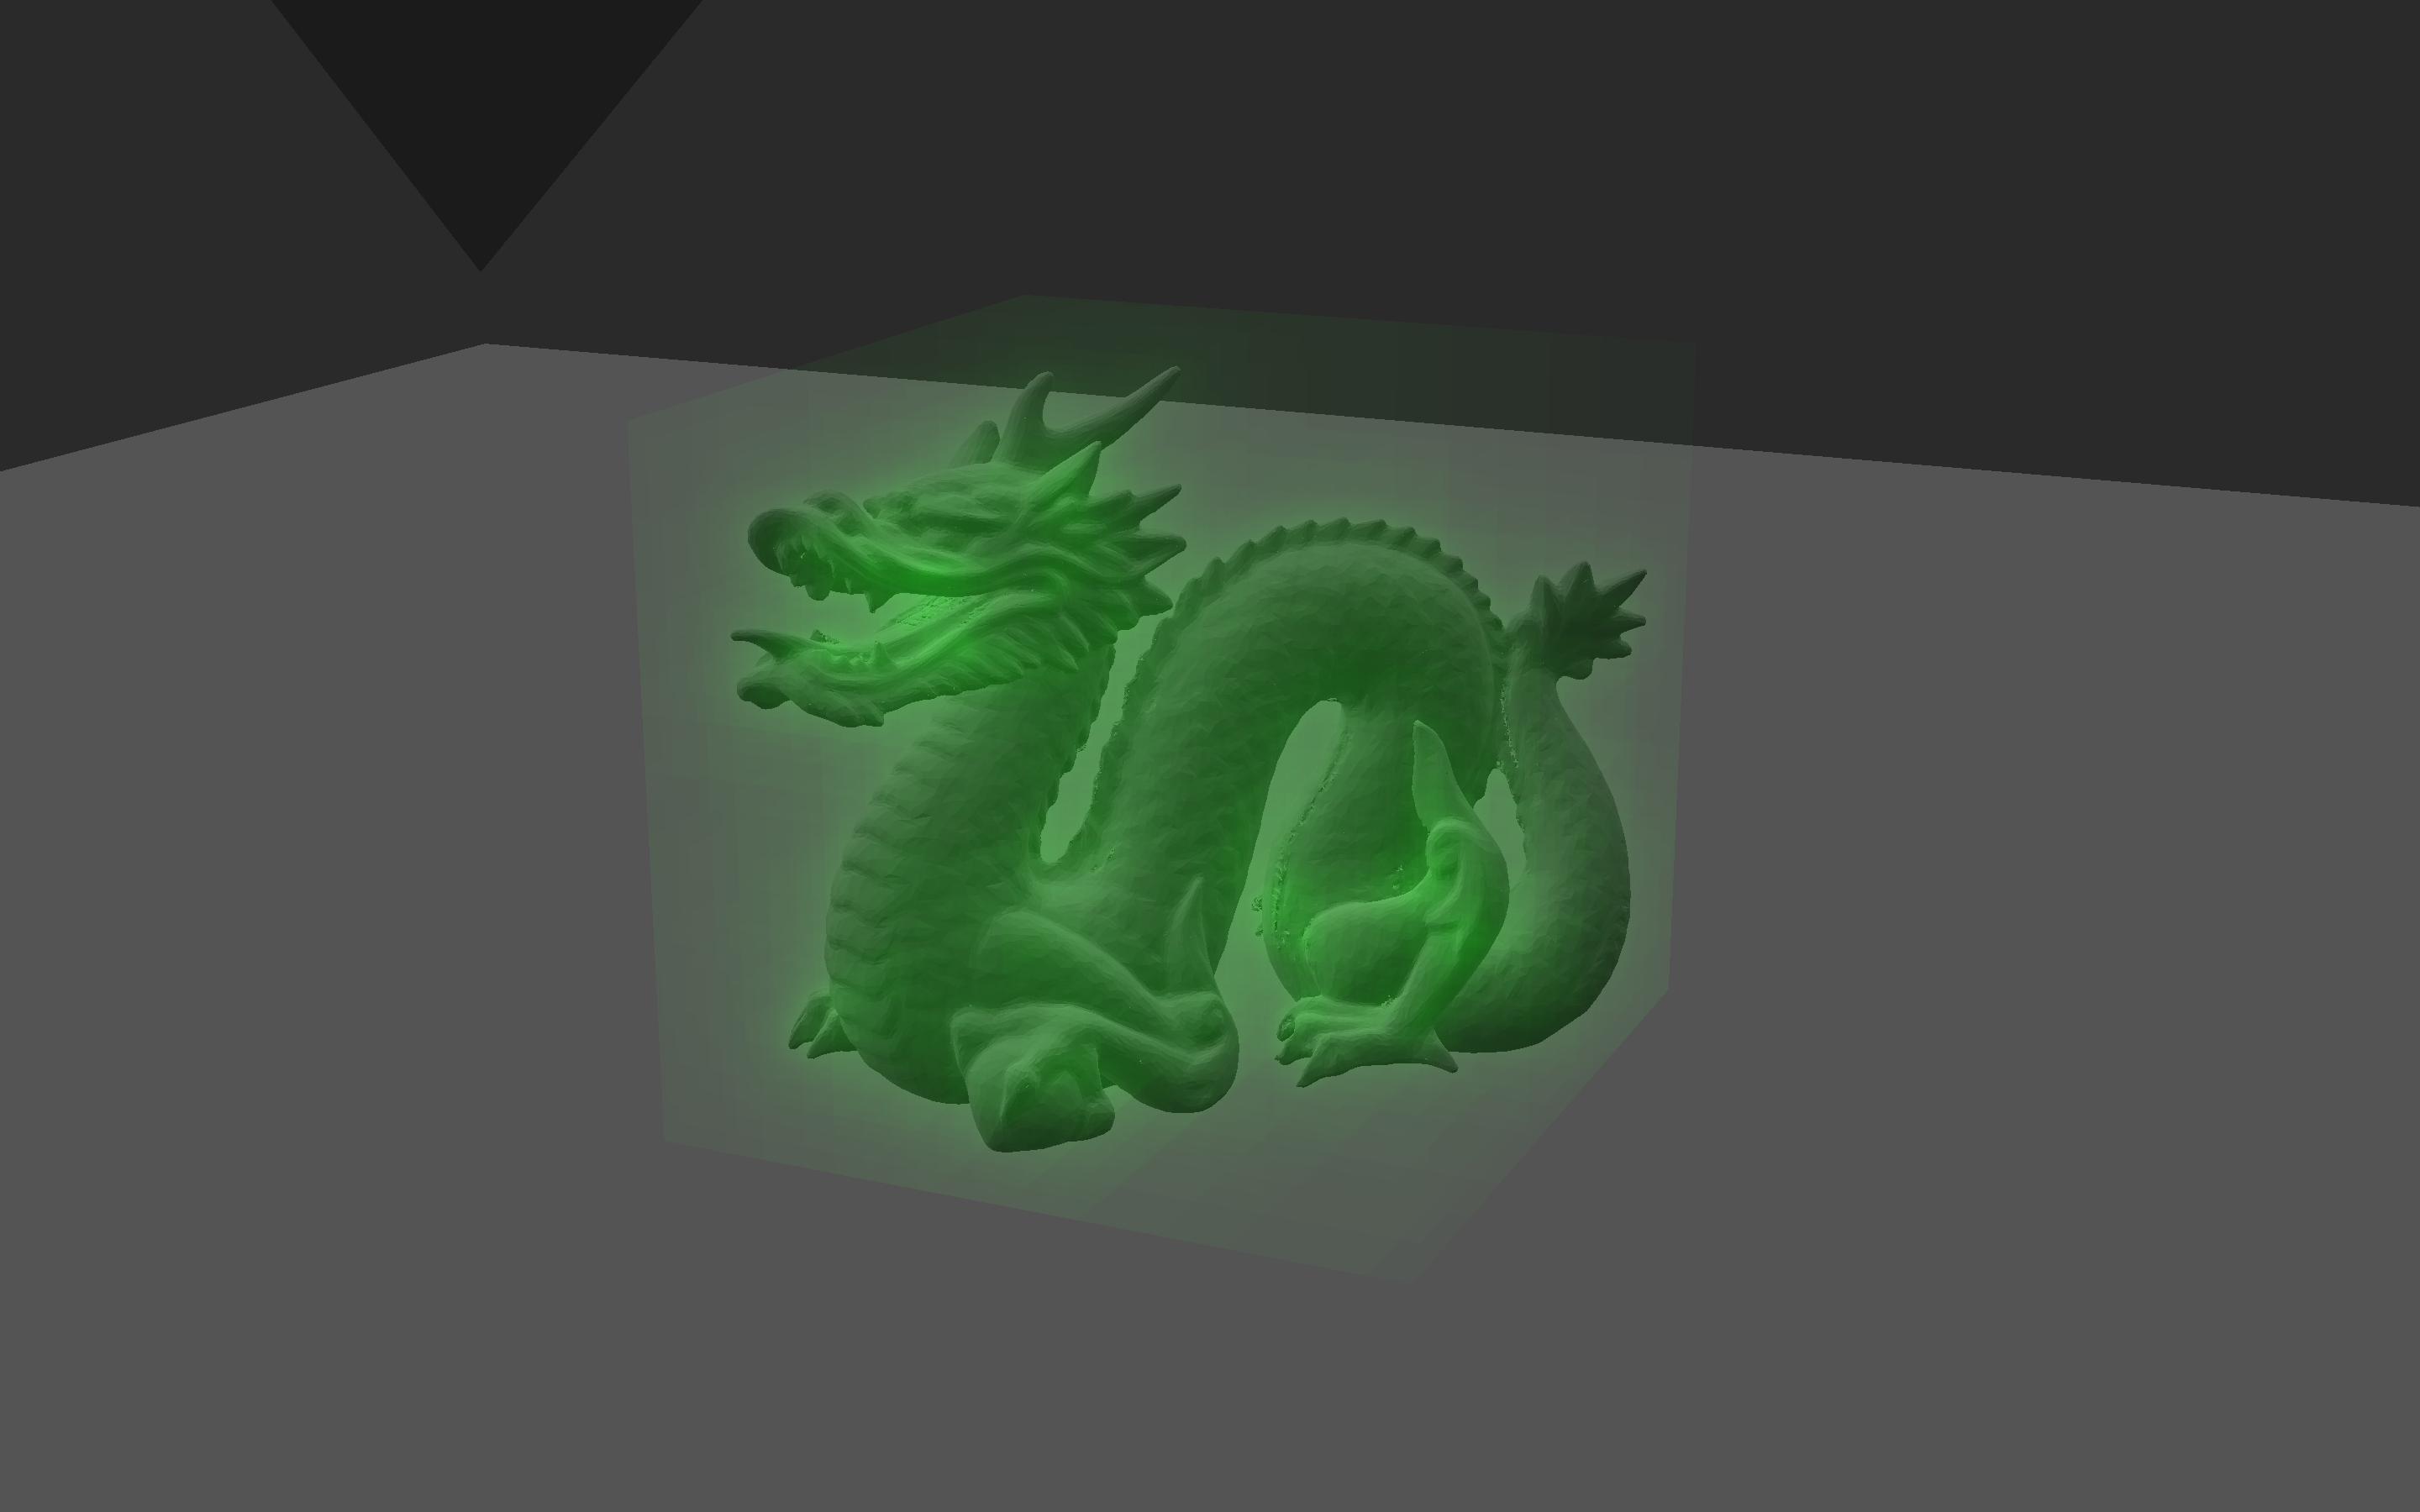
\includegraphics[width=0.8\columnwidth]{stats_octree_loops_optimized.png}
    \caption{
        Stanford dragon rendered with the sub-node access lists showing
        the linear number of octree loops required to browse.
    }
    \label{fig:stanford_dragon_with_access_list}
\end{figure}

Now this list is an integer list of the sub-nodes' id in
\textit{subnodeOffsets}. Therefore those 8 integers are in range $[0;8[$. That
means they can all be packed in an single \textit{uint32\_t} as shown on
Figure~\ref{code:subnode_access_unpacking}:

\begin{figure}[H]
    \centering
    \begin{lstlisting}[morekeywords={uint32_t}]
uint32_t const subnodeId =
    ((subnodeAccessList >> ((i++) * 4)) & 0x7);
    \end{lstlisting}
    \caption{Octree sub-nodes access lists' unpacking}
    \label{code:subnode_access_unpacking}
\end{figure}

But octree nodes are now taking nearly twice more memory size, and so is going
to clobber the memory cache even more because accessing a bigger amount of
memory pages. The performance are easily proven on very simple scenes, but when it comes
to ones with more detailed meshes like shown one Figure~\ref{fig:stanford_dragon}, the cache
clobber can actually drop rendering performances (Figure~\ref{table:subnode_access_list}).

\begin{figure}[h]
    \centering
    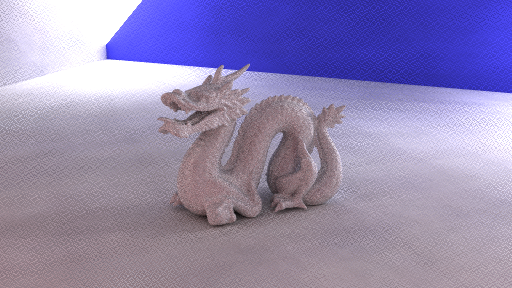
\includegraphics[width=0.8\columnwidth]{render_stanford_dragon.png}
    \caption{Stanford dragon (100k triangles)}
    \label{fig:stanford_dragon}
\end{figure}

This is where the second stage of this optimization come in. Instead of storing
all access lists in a node, we just store the node's sub-node mask into the
node struct. Because there an octree node can only have 8 sub-nodes, that
means the octree mask can actually have $2^8 = 256$ distinct possible values.
So we just have to precompute a constant array at compile-time that for a given sub-node mask
and a ray direction. Meaning this 32~bits integer array has $256 \times 8 = 2048$
cells. Then we can see with Figure~\ref{table:subnode_access_list} that this
improved optimization scales perfectly when it comes to more details meshes.

\begin{figure}[H]
    \centering
    \begin{lstlisting}[morekeywords={uint8_t,uint32_t}]
struct octree_node_t
{
    // the sub-nodes' offset from the octree root
    uint32_t subnodeOffsets[8];
    // the first primitive (mesh or triangle) id
    uint32_t primFirst;
    // the number of primitives
    uint32_t primCount;
    // the sub-node mask
    uint8_t subnodeMask;
    // the node's sub-node count
    uint8_t subnodeCount;
};
    \end{lstlisting}
    \caption{Octree node's structure with the sub-node mask.}
    \label{code:mask_access_list}
\end{figure}

\begin{figure}[H]
    \centering
    \begin{lstlisting}[morekeywords={uint8_t,uint32_t}]
node->subnodeMask = 0x00;
for (size_t i = 0; i < 8; i++) {
  node->subnodeMask |=
      ((node->subnodeOffsets[0] != 0) << i);
}
    \end{lstlisting}
    \caption{Algorithm that compute a node's sub-node mask.}
    \label{code:mask_access_list}
\end{figure}

\begin{figure}[H]
    \tiny
    \centering
    \begin{tabular}{ | l | c | }
        \hline
        Sub-nodes access lists optimization & Stanford Dragon \\
        \hline
        Disabled & 603.5ns \\
        With raw access lists & 617.7ns \\
        With sub-node mask & 528.6ns \\
        \hline
    \end{tabular}
    \caption{
        Octree node's sub-node access list optimization's average rendering
        time per ray.
    }
    \label{table:subnode_access_list}
\end{figure}
